\textbf{CP Violation and Weak Hadronic Interactions}

Observations of kaons and pions decaying at different rates led Cabibbo to propose quark mixing.

Quark mixing can happen at weak vertices through CKM matrix

\begin{center}
    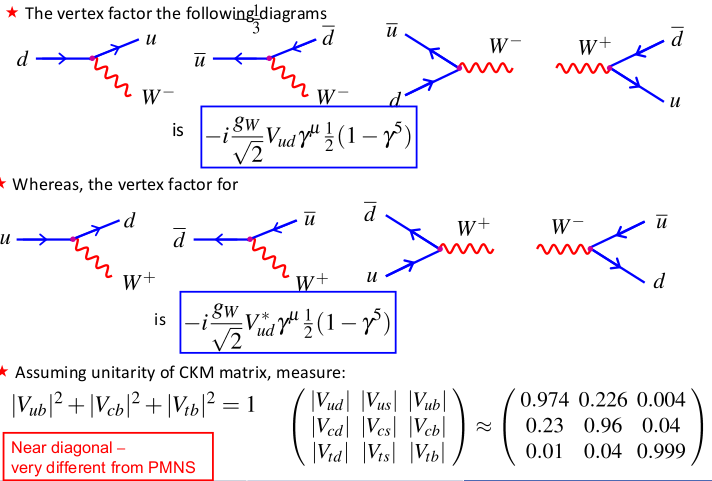
\includegraphics[width=\linewidth]{images/ckm_vertices.png}
\end{center}

CP violation gives things like $K_S, K_L, B_H, B_L$

\begin{center}
    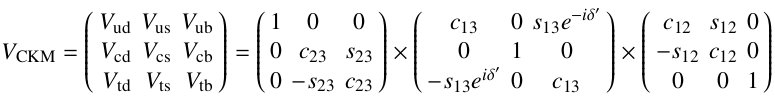
\includegraphics[width=\linewidth]{images/ckm_parametrization.png}
    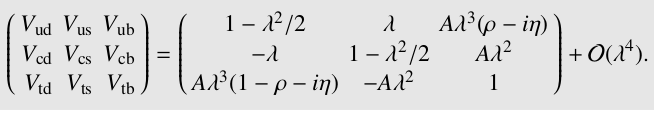
\includegraphics[width=\linewidth]{images/ckm_wolfenstein.png}
    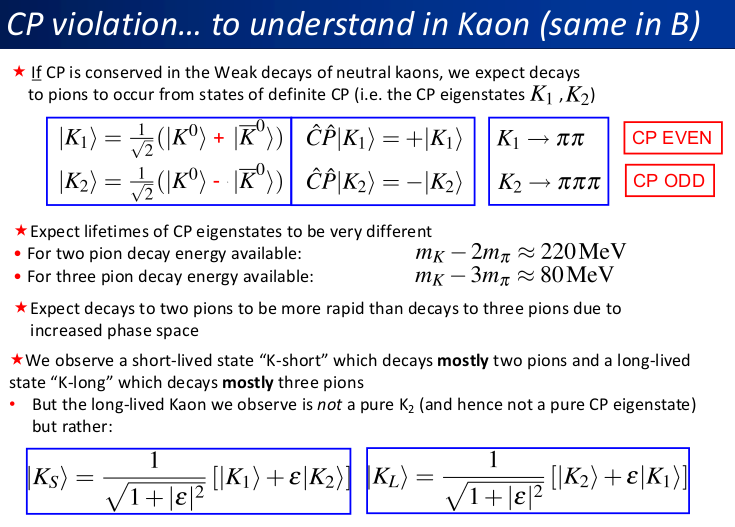
\includegraphics[width=\linewidth]{images/kshort_klong.png}

    $K_1$ is the 3-pion one, $K_2$ goes to 2 pions

    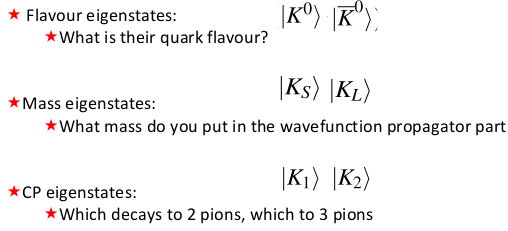
\includegraphics[width=\linewidth]{images/kaon_eigenstates.png}
\end{center}

In practice, $K_S \approx K_1, K_L \approx K_2$

It's the same kind of thing with neutral B mesons,

$(B^0, \bar{B}^0)$ flav. eigs., $(B_H, B_L)$ mass eigs
\begin{center}
    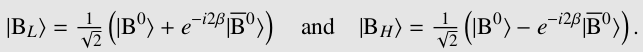
\includegraphics[width=\linewidth]{images/BH_BL.png}
\end{center}

$\sin(2\beta) = 0.685 \pm 0.032$

Wolfenstein params: $\lambda = 0.2253, A = 0.811, \rho = 0.13, \eta = 0.345$

Oscillations arise because natural mesons are produced as flavour eigenstates and decay as either flavour or CP eigenstates, but propagate as physical mass eigenstates.